%Preamble
\documentclass[12pt,a4paper]{article}        %Define text type and basic formatting
\usepackage[margin=1.25in]{geometry}
%\usepackage[document]{ragged2e}   %Text alignment https://www.overleaf.com/learn/latex/Text_alignment
\usepackage{microtype}  %Refined word breaks

\usepackage[utf8]{inputenc}     %Usage of UTF-8 for umlauts
\usepackage[ngerman]{babel}     %Paper language;
\pagenumbering{arabic}  % "Normal" page numbering
%Set line spacing to 1.5
% \usepackage{setspace}
% \onehalfspacing

%Citation and reference
\usepackage[backend=biber,
  style=authoryear,
  citestyle=authoryear-comp,
  hyperref=true,
  giveninits,    %Shorten first names to initial
  uniquename=init,    %prevent name disambiguation
  sorting=nyt,  % sort by name, year, title
  natbib,  %enable citep/citet(parentheses only around year)
  maxbibnames=99,  %show all names in bibliography (no influence on in-text citation)
  minbibnames=1  %show at least one name before et al
]{biblatex}   %REFERENCES https://www.overleaf.com/learn/latex/Bibliography_management_in_LaTeX
\addbibresource{references.bib}     %Lib file
\usepackage[nottoc,numbib]{tocbibind}   %add bibliography to toc

%page citation in text with colon: https://tex.stackexchange.com/questions/433122/changing-comma-in-textcite-to-colon
%\DeclareFieldFormat{postnote}{#1}
%\DeclareFieldFormat{multipostnote}{#1}
%\renewcommand\postnotedelim{\addcolon\addspace}

% Ensure "S." appears before page numbers in citations
\DeclareFieldFormat{postnote}{S.~#1}
\DeclareFieldFormat{multipostnote}{S.~#1}

% Handle comma between author and year and et al.
\renewcommand\nameyeardelim{\addcomma\space} %comma between author and year
%u.a. as et al.
\DefineBibliographyStrings{german}{%
  andothers = {et al.},
}
%Replace and/und with &
\renewcommand*{\finalnamedelim}{%
  \ifnumgreater{\value{liststop}}{2}{\finalandcomma}{}%
\addspace\&\space}%

% Easier inline citation -> \say{} command
\usepackage{dirtytalk} 

%images
\usepackage{graphicx}       %Required for adding images
\graphicspath{{images/}}    %image path
\usepackage{wallpaper}  %Page background img

\usepackage{parskip}        %Prevent indention of paragraphs
\usepackage{mathtools}    %required for math formulas
\usepackage{amssymb}    %mathematical symbols
\usepackage{listings}   %For code listings

%Use markdown in LaTex https://de.overleaf.com/learn/latex/Articles/How_to_write_in_Markdown_on_Overleaf
\usepackage[footnotes,definitionLists,hashEnumerators,smartEllipses,hybrid]{markdown}

\usepackage{titlesec}   %Style titles
\usepackage{fancyhdr}   %Header/footer
%\usepackage[bottom]{footmisc}   %Foot notes, at end of page

%Links
\usepackage[colorlinks,
  pdfpagelabels,
  pdfstartview = FitH,
  bookmarksopen = true,
  bookmarksnumbered = true,
  linkcolor = black,
  plainpages = false,
  hypertexnames = false,
  citecolor = black,
urlcolor = black]{hyperref}   %Hyperref pkg -> clickable links and TOC
\usepackage{csquotes}   % Autostyle quotes language-specific

%Font settings
\renewcommand{\familydefault}{\sfdefault}       %Text sans-serif
\renewcommand{\headrulewidth}{0pt}
\pagestyle{fancy}

%Footer
\fancyhf{}      %Clear all header/footer stylings
% \lfoot{\thedate\hspace{1pt}}
% \cfoot{Proposal Bachelorarbeit\\«Video- und bildbasierte Desinformation auf Social-Media-Plattformen in der Schweiz» (Arbeitstitel)} % Footnote
\rfoot{\thepage\hspace{1pt}}        %Add page number

%Title page settings
\usepackage{pdfpages}
\usepackage{titling}    %Title page styling
\title{«Analyse (audio-) visueller Desinformation auf Social-Media-Plattformen in der Schweiz» (Arbeitstitel)}        %Document Title
\author{Yannick Spriessler}     %Author of paper
\date{\today}     %Date of paper; ALTERNATIVE: \today

% Separate bibliography for images
% \defbibheading{imagecredits}{\section*{Bildverweis}}
% \addbibresource{img-references.bib}

%___________________________________________________________________________________________
%TITLE PAGE
\begin{document}
\begin{titlingpage} %Start titling page
  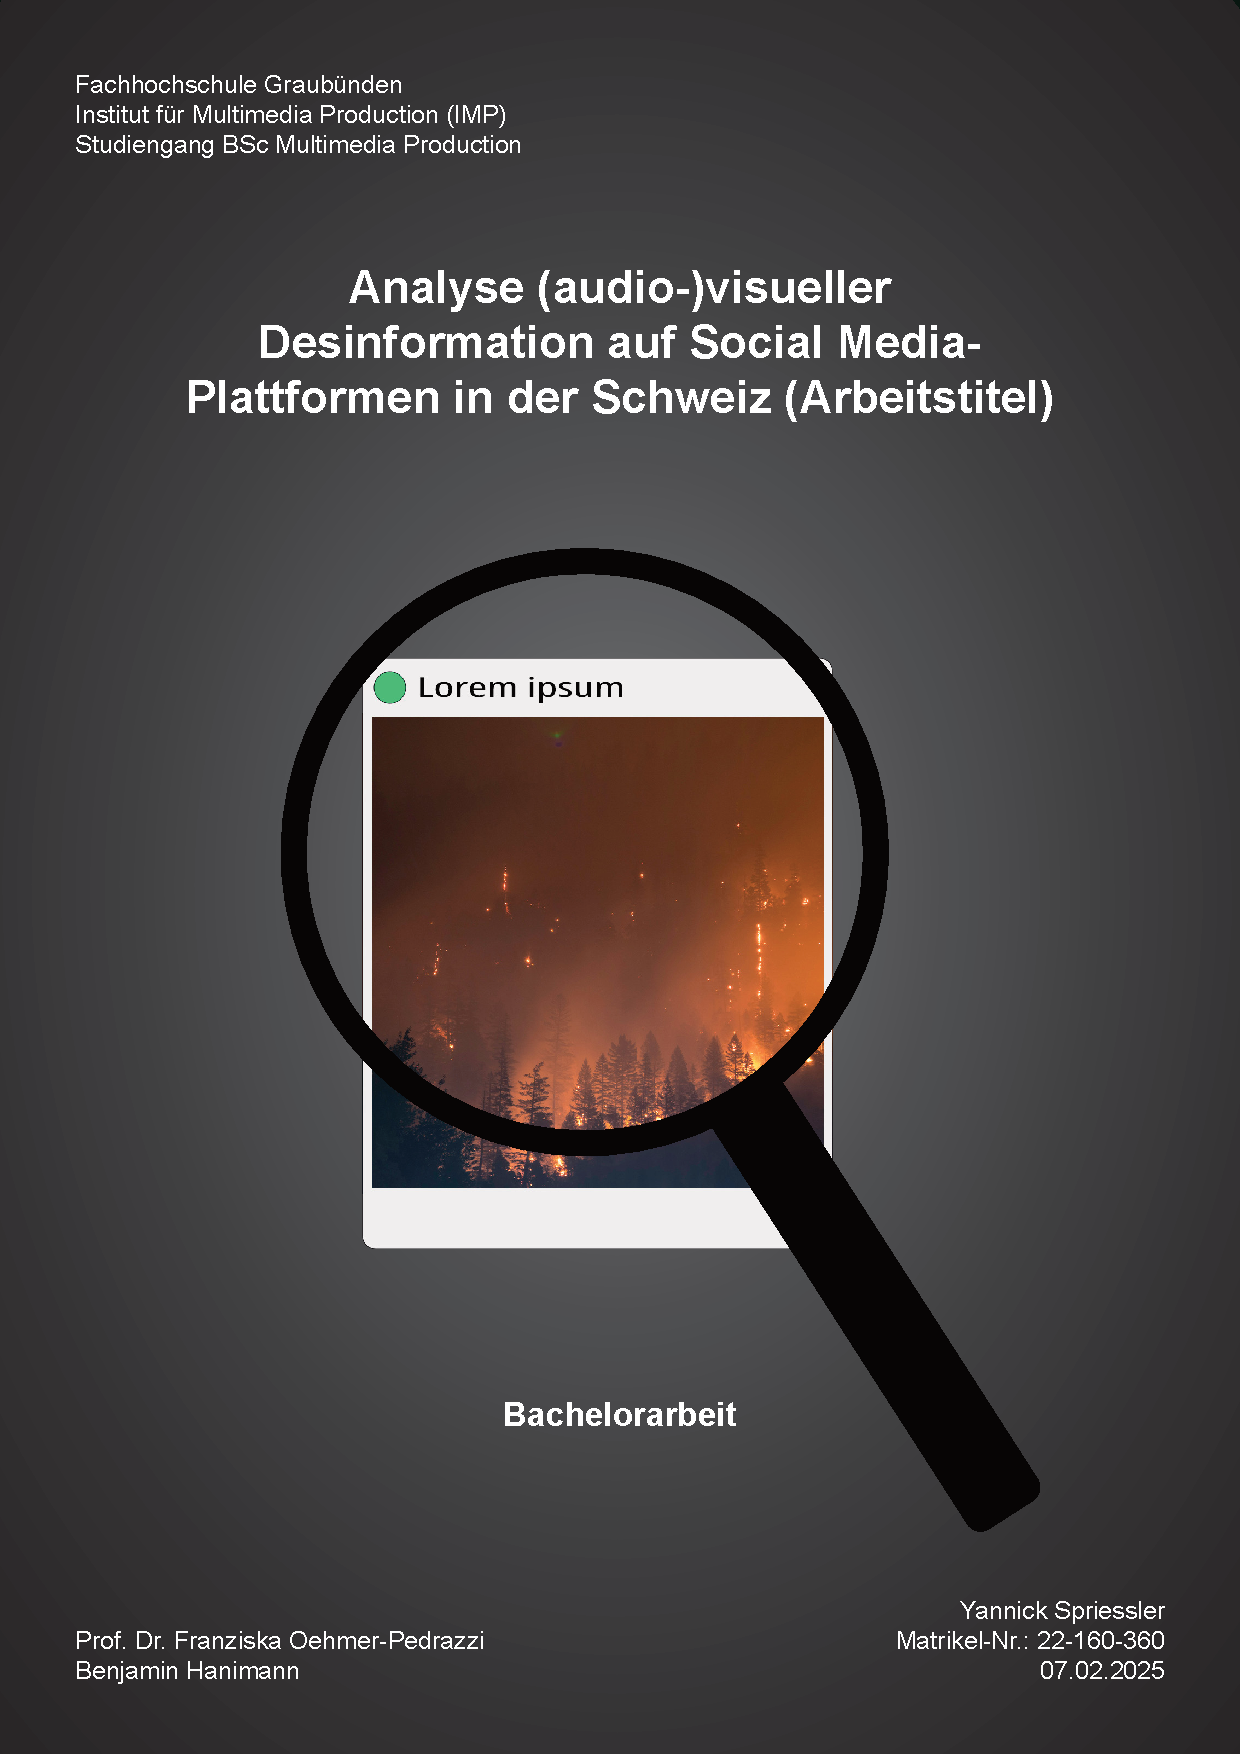
\includepdf{Titelblatt_Thesis}
  \nocite{howard_trees_2017}  %Citation for title page, only in image bibliography
\end{titlingpage}
\pagebreak      %Insert page break
%-----------------------------------------------
\renewcommand{\abstractname}{Abstract}
\begin{abstract}
  \setlength{\parindent}{0pt}  
    asdfghjk \\
\end{abstract}

\textbf{Keywords:} \textit{Desinformation, Social Media, audiovisuelle Inhaltsanalyse}


\textbf{Zitiervorschlag:}
\linebreak
%\frontmatter   %If foreword
\pagebreak
%TOC
\thispagestyle{empty}
\setcounter{page}{0}    %Set page no.
\tableofcontents        %Content index
\pagebreak
%-----------------------------------------------
%DOC

%\mainmatter    %Main part if foreword used
\section{Einleitung}
Spätestens seit den US-Wahlen 2016 hat der Begriff «Fake News» stark an Bedeutung gewonnen. Zwar handelt es sich dabei nicht um eine Neuerscheinung und falsche Informationen wurden lange vor der Entwicklung des Internets verbreitet \parencites[214]{allcott_social_2017}[247]{hohlfeld_schlechte_2020}[1]{khan_fake_2021}, dennoch ist das Problem unter anderem durch die Verbreitung über das Internet weiter stark angewachsen \parencites[214–215]{allcott_social_2017}[1]{khan_fake_2021}[1]{lazer_science_2018}[4]{ceron_fake_2021}. \\
Aufgrund der sozialen Medien und der Möglichkeit, innerhalb kürzester Zeit Videos und Bilder zu produzieren, können heute sehr schnell audiovisuelle Falschinformationen verbreitet werden. Diese stellen nicht nur ein Problem für die individuellen Rezipierenden dar, sondern gefährden dabei auch politische und gesellschaftliche Prozesse.

Die Bachelorarbeit befasst sich damit, welche inhaltlichen und gestalterischen Merkmale audiovisuelle und bildbasierte Desinformation auf Social-Media-Plattformen in der Schweiz aufweist. \\
Ziel der Arbeit ist es zum einen, herauszufinden, ob es mögliche Muster und
Strategien hinter der Produktion der Inhalte gibt. Zum anderen soll auch ein
allgemeines Verständnis über die entsprechenden Inhalte gewonnen werden. \\
Die Erkenntnisse der Bachelorarbeit werden anschliessend verwendet, um darauf basierend eine interaktive Aufklärungsplattform zu gestalten.

\subsection{Relevanz}
\textbf{Gesellschaft}
\linebreak
Im Jahr 2024 betrug der Anteil der Social-Media-Nutzenden in der Schweiz knapp 80 \%. Weiter informiert sich ein bedeutender Anteil der europäischen Bevölkerung über das Internet, eine Mehrheit verwendet Social Media primär für Nachrichten und Unterhaltung \parencite[21ff]{we_are_social_anteil_2024}. Gemäss der JAMES-Studie 2024 \parencite[40]{kulling-knecht_james_2024} informiert sich 2024 etwa die Hälfte der Jugendlichen täglich oder mehrmals pro Woche auf sozialen Plattformen. \\
Somit wird durch Social-Media-Inhalte ein Grossteil der Schweizer Bevölkerung erreicht. Dadurch können desinformierende Inhalte potenziell einen grossen Einfluss auf die Bevölkerung und ihre (politische) Meinungsbildung haben \parencites[18]{grujic_warnhinweise_2024}[258]{hohlfeld_schlechte_2020}[1f]{khan_fake_2021}, insbesondere wenn Social-Media-Plattformen auch als Informationsquelle zu politischen und gesellschaftlichen Themen dienen.

\textcite{grady_neural_1998} haben gezeigt, dass sich Rezipierende besser und länger an visuelle Inhalte erinnern können als an Worte. Eine weitere Untersuchung fand einen Zusammenhang zwischen dem Konsum von Videos und der Möglichkeit der Nutzenden, auf diese zu reagieren \parencite[242]{khan_social_2017}. Inhalte mit Partizipationsmöglichkeit scheinen ausserdem den weiteren Konsum (\textit{information seeking}) zu befeuern \parencite[243]{khan_social_2017}. \\
Insofern kann davon ausgegangen werden, dass audiovisuelle Desinformation eine besondere Gefahr darstellt. 

\textbf{Politik}
\linebreak
\textcite[258]{hohlfeld_schlechte_2020} schreiben Desinformation die Fähigkeit zu, demokratische Gesellschaften \say{durch Inhalte, die Angst und Verunsicherung schüren, [\ldots] [sowie, d. Verf.] durch die Schwächung der seriösen Institutionen der Erkenntnisbeschaffung und [\ldots] durch Normverschiebungen des politisch Sagbaren} zu destabilisieren. \parencite[vgl.\ auch][1]{khan_fake_2021}.

Eine Marketingfirma fand 2016 heraus, dass Fake-News-Seiten für die Verbreitung ihrer Inhalte fast komplett  von Facebook abhängig sind. Während solche Seiten 50 \% der Websitebesuche von Facebook erhalten, lagen seriöse Medien bei etwa 20 \%.\parencites{wong_almost_2016}[zit.\ nach][1]{khan_fake_2021}[vgl.\ auch][212]{allcott_social_2017}. \\
Facebook und weitere Social-Media-Plattformen können somit als starke Treiber von Desinformation verstanden werden \parencite{wong_almost_2016}. In Anbetracht der jüngsten Tendenz, Einordnungen durch Faktencheck-Organisationen auf den Meta-Plattformen einzustellen \parencites{isaac_meta_2025}{meta_transparency_centre_penalties_2025}, ist es für die Nutzenden deshalb umso wichtiger, Inhalte bezüglich ihres Wahrheitsgehalts korrekt einordnen zu können. 

Gemäss dem \textcites{bundesministerium_des_innern_und_fur_heimat_desinformation_2022}\parencite[zit.\ nach][15]{teetz_social-media-post_2023} kann Desinformation in einigen Fällen sogar als Bedrohung der nationalen Sicherheit verstanden werden. \\
Die Schweiz hat mit ihrer direkten Demokratie ein weltweit einzigartiges politisches System, in keinem anderen Staat hat die Bevölkerung so viele Mitbestimmungsrechte \parencite[2]{sager_politische_2017}. Es ist deshalb zwingend notwendig, dass diese ihre politischen Entscheide aufgrund von korrekten Fakten und eigener politischer Entscheidung treffen kann, ohne von Desinformation beeinflusst zu werden \parencite[26]{vogler_wahrnehmung_2021}\parencite[vgl.\ auch][14f]{colomina_impact_2021}. Auch wenn über die tatsächliche Gefährdung der Schweizer Politik durch Desinformation bisher noch wenig bekannt ist, scheint die Schweiz als Staat vergleichsweise widerstandsfähig zu sein (ebd.).\\
Durch das Wissen der Plattform-Nutzenden über Desinformation und die Mechanismen der Social-Media-Plattformen sowie die Fähigkeit, falsche von echten Tatsachen zu unterscheiden, kann diese Gefahr weiter verringert werden.

\textbf{Wissenschaft}
\linebreak
Soziale Medien funktionieren fundamental anders als traditionelle Medien. Nachrichten und andere Inhalte können ohne faktische Einordnung oder inhaltlichen Kodex weltweit geteilt werden \parencite[211]{allcott_social_2017}. Die journalistischen Kriterien wie \say{Unabhängigkeit,  Ausgewogenheit, Vielfalt, Verständlichkeit und Unterhaltsamkeit}\parencite[9]{grujic_warnhinweise_2024} werden nicht überprüft. Besonders in Krisenzeiten sind die Nutzenden besonders anfällig für Falschinformationen \parencite[vgl.][2]{ceron_fake_2021}. \\
Social-Media-Plattformen und ihre entsprechenden Algorithmen zur Inhaltsauswahl basieren neben den Interaktionen der Nutzenden untereinander in ihrer Funktionsweise vor allem auf der Generierung von Aufmerksamkeit \parencites[vgl.][220]{schmidt_meinungsbildung_2022}[493]{behnke_manipulation_2018}. \\
Durch die Verbreitung eines Inhaltes wird zwangsläufig die Kapazität der Nutzenden für die Verarbeitung anderer Inhalte geschmälert \parencite[248]{hohlfeld_schlechte_2020}.

Die Wissenschaft kennt das Potenzial und die Gefahr von Social-Media-Plattformen, durch Fragmentierung und das Anzeigen bestimmter Inhalte Filterblasen zu schaffen und die Gesellschaft zu spalten – dieser Effekt konnte jedoch bisher nicht tatsächlich bewiesen werden \parencite[220]{schmidt_meinungsbildung_2022}.

Als Massnahme gegen Desinformation werden oft Faktenchecks eingesetzt. Deren Wirksamkeit wird allerdings immer wieder in Frage gestellt \parencites[1095]{lazer_science_2018}[4f]{ceron_fake_2021}. \say{(\ldots) people prefer information that confirms their preexisting attitudes (selective exposure), view information consistent with their preexisting beliefs as more persuasive than dissonant information (confirmation bias), and are inclined to accept information that pleases them (desirability bias).} \parencites[1095]{lazer_science_2018}\parencite[vgl.\ auch][18]{grujic_warnhinweise_2024}. Faktenchecks könnten in einigen Fällen sogar kontraproduktiv sein, wenn  die Falschinformation wieder aufgefrischt wird und dadurch eher hängenbleibt als die faktische Einordnung (ebd.). Umso wichtiger ist es, dass die Rezipierenden die medialen Artefakte möglichst selbst beurteilen können.

\subsection{Forschungsfrage}
Folgende Fragestellung wird in der Bachelorarbeit behandelt:

\begin{quote}
  Welche inhaltlichen und gestalterischen Merkmale weist visuelle und audiovisuelle Desinformation auf Social-Media-Plattformen in der Schweiz auf?
\end{quote}
\color{red}Begründung für Forschungsfrage.

\color{red}Aufbau der Arbeit 
\color{black}
\pagebreak
\section{Forschungsstand zur Desinformation}

%Zusammenfassung des Kapitels

\subsection{Begriffsdefinition}

Beispielsweise durch die Präsidentschaft des US-Präsidenten Donald Trump (2017–2021) oder den Brexit hat der Begriff «Fake News» weltweit an Bedeutung gewonnen \parencites[1f]{hohlfeld_schlechte_2020}[1]{marx_fake_2020}. \\
In der Literatur existieren verschiedene Definitionen des Begriffes. \textcite[246f]{hohlfeld_schlechte_2020} vertreten beispielsweise die Haltung, dass «Fake News» als Begriff für desinformierende Inhalte gleichbedeutend sind mit dem politischen Propagandabegriff. In den letzten Jahren wurde allerdings auch oft argumentiert, dass «Fake News» lediglich als politischer Begriff gewertet und im wissenschaftlichen Kontext stattdessen von (aktueller) Desinformation gesprochen werden sollte \parencites[3]{bontridder_role_2021}{habgood-coote_stop_2019}[148]{marx_fake_2020}. Egelhofer \& Lecheler \parencite[zit.\ nach][148]{marx_fake_2020} differenzieren zwischen «Fake News» als Genre für Falschinformationen und «Fake News» als Label im Sinne einer politischen Instrumentalisierung zur Diskreditierung von Medien und Institutionen.\\
In Anlehnung an \textcite{marx_fake_2020} und in Abgrenzung zum politischen Label wird in dieser Bachelorarbeit der Begriff «Desinformation» verwendet.

In der Wissenschaft gibt es bisher keine einstimmige Definition für Desinformation. 
\textcite[148f]{marx_fake_2020} benennen ein Theoriendefizit, basierend auf widersprüchlichen Definitionen sowie nicht nachvollziehbaren Definitionskriterien.\\
Laut \textcite[1094]{lazer_science_2018} handelt es sich bei Desinformation um \say{fabricated information that mimics news media content in form but not in organizational process or intent. Fake-news outlets, in turn, lack the news media’s editorial norms and processes for ensuring the accuracy and credibility of information.}
\textcite[213]{allcott_social_2017} sprechen von \say{(\ldots) news articles that are intentionally and verifiably false, and could mislead readers.} \parencites[vgl.\ auch][140]{tandoc_jr_defining_2018}[1094]{lazer_science_2018}.\\
Diese Definition kann nicht nur auf News-Artikel angewendet werden, sondern auch auf andere mediale Artefakte \parencite[3]{bontridder_role_2021} \parencite[vgl.\ auch][16]{reuter_fake_2019}. \textcite[1]{marx_fake_2020} definieren aktuelle Desinformation als \say{Kommunikation wissentlich und empirisch falscher Informationen zu neuen und relevanten Sachverhalten mit dem Anspruch auf Wahrheit.} Sie stützen sich dabei auf folgende Kriterien:

\begin{itemize}
  \item \textbf{(Visuelle) Kommunikation}: Eine wahrheitsfähige Mitteilung mit darstellendem Gehalt, welche einen Wirklichkeitsausschnitt abbildet. Dies bezieht sich nicht nur auf sprachliche, sondern auch auf visuelle Mitteilungen \parencite[151]{marx_fake_2020}.
  \item \textbf{Aktualitätsbezug}: \say{(\ldots) überraschende Themen mit (potenziell) großer Auswirkung auf die Gesellschaft. So ermöglicht sie ihrem Publikum die Ausbildung von (wenn auch empirisch unzutreffenden [\ldots]) Erwartungen und dadurch die Orientierung in einer komplexen Welt.} \parencite[152]{marx_fake_2020}.
  \item \textbf{Wahrheitsanspruch}: Aktuelle Desinformation beansprucht für sich, dass sie (vorgetäuscht) wahr ist. In diese Betrachtung werden sowohl Produzierende wie auch Rezipierende des Inhaltes miteinbezogen. Hierbei gilt, ob es für externe Beobachtende plausibel ist, dass Rezipierende die Nachricht als wahr betrachten \parencite[153]{marx_fake_2020}.
  \item \textbf{Unwahrheit}: Der desinformierende Inhalt besitzt irreführendes Potenzial, da er empirisch falsch ist und somit den zuvor beanspruchten Wahrheitsgehalt nicht einlöst. \parencite[154]{marx_fake_2020}.
  \item \textbf{Unwahrhaftigkeit}: Die Produzierenden sind sich der Tatsache bewusst, dass ihre Mitteilungen falsch sind. \parencite[156]{marx_fake_2020}
  \item \textbf{Täuschungsabsicht}: Falsche Tatsachen werden vorsätzlich und bewusst verbreitet. Dabei spielt es keine Rolle, ob diese der gezielten Verbreitung von Falschinformationen dienen sollen oder beispielsweise zu Clickbait-Zwecken eingesetzt werden \parencites[157]{marx_fake_2020}[vgl.\ auch][2]{khan_fake_2021}. 
\end{itemize}

Desinformation muss abgegrenzt werden von weiteren verwandten Themen und Begriffen:

\begin{itemize}
  \item \textbf{Missinformation}: Missinformation \say{ (\ldots) refers to false, inaccurate, or misleading information that is shared without any intent to deceive.} \parencite[2]{bontridder_role_2021}. \citeauthor{marx_fake_2020} grenzen Missinformation anhand des Unwahrhaftigkeitskriteriums ab, indem es sich bei Missinformation gemäss ihrer Definition um eine unwissentliche Fehlinformation handelt \parencite[156]{marx_fake_2020}, welche ohne Täuschungsabsicht verbreitet wird \parencite[vgl.\ auch][15]{grujic_warnhinweise_2024}.
  \item \textbf{Satire}: Satire ist nach \textcite[154]{marx_fake_2020} erkennbar an einer klaren Quelle (beispielsweise ein Satiremagazin) sowie bestimmten Text- und Stilmerkmalen und grenzt sich von Desinformation ab durch den Verzicht auf den Wahrheitsanspruch. Diese Einschätzung wird ebenfalls durch externe Beobachtende getroffen.\\
  Weitere Merkmale sind humoristische oder übertriebene Darstellungen \parencites[141]{tandoc_jr_defining_2018}[2]{khan_fake_2021}, obwohl diese auch in seriösen und korrekten Nachrichten verwendet werden können.
  \item \textbf{Gerücht}: Ein Gerücht zeichnet sich dadurch aus, dass sein Wahrheitsgehalt (noch) nicht überprüft ist \parencite[155]{marx_fake_2020}. Der Wahrheitsgehalt von Desinformation lässt sich jederzeit prüfen.
  \item \textbf{Verschwörungstheorie}: Rosnow \& Kimmel \parencite[zit.\ nach][197]{krafft_disinformation_2020} definieren Verschwörungstheorien (Rumors) als \say{an unverified proposition for belief that bears topical relevance for persons actively involved in its dissemination.} (ebd.). \textcite[197]{krafft_disinformation_2020} halten eine persönliche Betroffenheit sowie Informationsunsicherheit als Bedingungen für eine Verschwörungstheorie fest.\\
  Von Desinformation unterscheidet sich eine Verschwörungstheorie dadurch, dass sie meist auch von denjenigen geglaubt wird, welche zu ihrer Verbreitung beitragen \parencite[156]{marx_fake_2020}.
  \item \textbf{Fake News}: Zum einen wird der Begriff im politischen Kontext als abwertendes Label verwendet für Nachrichten, welche nicht nach dem Willen der politischen Akteurinnen und Akteure berichten \parencite[3]{tandoc_jr_facts_2019}.\\
  Zum anderen handelt es sich bei «Fake News» um eine Unterkategorie der Desinformation, welche spezifisch Nachrichtenartikel bezeichnet, die Falschinformationen beinhalten und so aufbereitet sind, dass sie für echt gehalten werden (können) (ebd.).
\end{itemize}

\citeauthor{marx_fake_2020} haben in ihrer Arbeit eine Begriffsdefinition für aktuelle Desinformation aufgestellt, welche den Term klar definiert und von anderen Kategorien von Falschinformationen abgrenzt. In dieser Bachelorarbeit wird nachfolgend ihre Definition zur Beurteilung von Desinformation angesetzt.
\subsubsection{Was aktuelle Desinformation ist}
Viele Publikationen halten fest, dass aktuelle Desinformation kein neues Phänomen ist \parencites[vgl.\ bspw.][2]{tandoc_jr_facts_2019}[214]{allcott_social_2017}[1094]{lazer_science_2018}. \textcite[214]{allcott_social_2017} nennen als eines der ältesten Beispiele den \textit{Great Moon Hoax} von 1835.

Seit in den letzten 20 Jahren Social-Media-Plattformen aufgekommen sind, hat sich die traditionelle Informationsverbreitung stark ins Internet verlagert \parencites[211]{allcott_social_2017}[147]{marx_fake_2020}[138]{tandoc_jr_defining_2018}[1094]{lazer_science_2018}. Diese Plattformen erlauben es den Nutzenden, auf sehr einfache Art und ohne grosse Hindernisse Informationen online mit der gesamten Nutzerbasis zu teilen \parencites[1]{vogler_wahrnehmung_2021}{lazer_science_2018}. Informationen zu aktuellen Ereignissen können so ohne inhaltliche Richtlinien, Einordnungen oder Faktenkontrollen potenziell weltweit verbreitet werden \parencites[147]{marx_fake_2020}[211]{allcott_social_2017}[4]{ceron_fake_2021}[165f]{wahl_fake_2021}. \say{An individual user with no track record or reputation can in some cases reach as many readers as Fox News, CNN, or the New York Times.} \parencite[211]{allcott_social_2017}.

Mittlerweile informiert sich weltweit ein Grossteil der Bevölkerung auf sozialen Plattformen oder anderweitig online über aktuelle Geschehnisse \parencite[212]{allcott_social_2017}. Auch in der Schweiz nutzt mehr als die Hälfte der Bevölkerung soziale Medien zu Unterhaltungs- und Informationszwecken \parencite[21ff]{we_are_social_anteil_2024}. Nutzende, welche auf Social Media Inhalte zu aktuellen Vorkommnissen teilen, werden so journalistisch tätig, auch ohne sich dessen immer bewusst zu sein \parencite[139]{tandoc_jr_defining_2018}. Professionelle Journalisten und Medienhäuser sind diesem Trend in den letzten Jahren gefolgt und nutzen die Plattformen mittlerweile ebenfalls gezielt zur Verbreitung ihrer Inhalte (ebd.).

Die grosse Freiheit, welche diese Liberalisierung der Inhaltsverbreitung bietet, lässt gleichzeitig Raum für Missbrauch und die Verbreitung von Falschinformationen \parencite[4]{ceron_fake_2021}.\\ 
Seit 2016 ist vor allem in den USA das Mass an Desinformation stark angestiegen, bedingt durch den Wahlkampf von US-Präsident Donald Trump \parencites[1094f]{lazer_science_2018}{allcott_social_2017}[147]{marx_fake_2020}[147]{tandoc_jr_defining_2018}. \textcite[1094f]{lazer_science_2018} konstatieren einen historischen Tiefpunkt in der Glaubwürdigkeit in die öffentlichen Medien. Durch parteipolitische Polarisierung und geringere Toleranz für andere Meinungen durch Social-Media-Inhalte ist ein massiver Nährboden entstanden für die Verbreitung von Desinformation (ebd.).\\
Während der Covid-Pandemie 2020 wurde ebenfalls ein starker Anstieg an Desinformation auf den sozialen Medien verzeichnet, beispielsweise zu den neu entwickelten Impfstoffen \parencite[2]{khan_fake_2021}. \Textcite[2]{ceron_fake_2021} nennen als Ursache die vorherrschende Unsicherheit, welche die Verbreitung der Inhalte weiter befeuerte \parencite[vgl.\ auch][22f]{zoglauer_konstruierte_2021}. \\

Die Schweiz galt lange als vergleichsweise resistent gegen Desinformation \parencite[26]{vogler_wahrnehmung_2021}. Jedoch lässt sich auch hier seit 2021 ein Anstieg verzeichnen. Für die Schweiz gaben 2021 etwa ein Viertel der befragten Personen an, oft oder sehr oft auf Desinformation zu stossen (ebd.). In einer OECD-Studie von 2024 zeigte sich ausserdem, dass die Schweizer Bevölkerung in der Bewertung von Desinformation vergleichsweise schlecht abschnitt \parencite{wyl_schweizerinnen_2024}.

\subsubsection{Der Einfluss generativer künstlicher Intelligenz auf die Erstellung von Desinformation}
Vor allem seit der kommerziellen Veröffentlichung von OpenAI’s ChatGPT Ende 2022 hat das Thema generative künstliche Intelligenz an Bedeutung gewonnen. Der Bereich der Online-Desinformation bildet hier vor allem eine Schnittmenge mit generierten Bildern und Deepfake-Videos (beispielsweise \say{a false depiction of someone saying or doing something they never did} \parencite[5]{birrer_what_2024}), welche oftmals schwer erkennbar sind \parencites[7]{montasari_artificial_2022}. \say{More recently, developments in AI have further expanded the possibilities to manipulate texts, images, audios and videos, with the two latter types of content becoming increasingly realistic.} \parencite[4]{bontridder_role_2021}. \\
Befürchtungen zur Verbreitung KI-generierter Desinformation umfassen beispielsweise die Verletzung der Persönlichkeitsrechte durch die Falschdarstellung von Personen oder die gezielte, hyperpersonalisierte Verbreitung von Falschinformationen während politischer Wahlen oder Abstimmungen \parencite[56, 64f]{kertysova_artificial_2018}.\\ 
Zur effektiven Gefahr und Verbreitung von Deepfakes und KI-generierten Bildern sind bisher jedoch noch nicht genügend Erkenntnisse vorhanden. \parencite{birrer_what_2024}.

\subsection{Studien zu aktueller Desinformation}
\subsubsection{Wer verbreitet Desinformation?}
~\label{theory_disseminents}
% Ursprung
Die meisten Bürgerinnen und Bürger moderner Demokratien informieren sich nicht selbst aktiv über Themen wie Politik und die Gesellschaft, sondern ihr Wissensstand ist abhängig von den zur Verfügung stehenden Informationen der \say{information supply chain}. Diese wird bespielt mit journalistisch oder anderweitig medial aufbereiteten Inhalten, welche von den leitenden Akteurinnen und Akteuren der Gesellschaft ausgehen \parencite[69]{lecheler_disinformation_2022}.

% generelle Motivation hinter der Verbreitung
Da die Produktion von Desinformation einen bewussten Akt der Täuschung darstellt, kann davon ausgegangen werden, dass es schwierig ist, tatsächliche Aussagen über die Produzierenden zu treffen \parencite[73]{lecheler_disinformation_2022}. \textcite[39]{pennycook_lazy_2019} benennen als Grundmotivation jedoch bereits in ihrer Definition von Desinformation \say{highly salient [\ldots] fabricated claims that are created to spread on social media.}. Die Literatur nennt zumeist zwei klare Motive zur Produktion von Desinformation: finanzielle Anreize oder politische und ideologische Überlegungen.

Gehen Inhalte auf Social Media viral und werden einer grossen Menge an Nutzenden angezeigt, so generiert dies oft finanziellen Umsatz \parencites[217]{allcott_social_2017}[3]{tandoc_jr_facts_2019}[157]{marx_fake_2020}, indem beispielsweise auf externe Artikel verlinkt wird, welche dann Werbeanzeigen beinhalten. \textcite[76]{lecheler_disinformation_2022} weisen hier etwa auf Journalistinnen und Journalisten oder Medienhäuser hin, welche bewusst desinformierende Taktiken einsetzen, um durch Clickbaiting oder besonders polarisierende Inhalte mehr Umsatz zu generieren. \\
DOch nicht nur journalistische Akteurinnen und Akteure verwenden Desinformation aus finanziellen Gründen, sondern auch Privatpersonen. Ein berühmtes Beispiel stammt von den US-Wahlen 2016, als eine Gruppe Jugendlicher in Mazedonien massenweise Desinformation verbreitet hat, was ihnen Tausende von Dollars einbrachte \parencites[217]{allcott_social_2017}[vgl.\ auch][]{subramanian_meet_2017}[3]{tandoc_jr_facts_2019}. \textcite[217]{allcott_social_2017} erwähnen als weiteres Beispiel Paul Horner, welcher aus Profitgründen massenweise Desinformation auf Social Media geteilt hat \parencite[vgl.\ auch][]{dewey_facebook_2016}.

Als zweiter Motivationstreiber gelten ideologisch motivierte Versuche, Einfluss auf die politische Meinungsbildung zu nehmen und demokratische Institutionen zu schwächen \parencites[225]{schmidt_meinungsbildung_2022}[75]{lecheler_disinformation_2022}[157]{marx_fake_2020}. So werden zum Beispiel oftmals Politikerinnen und Politiker diskreditiert \parencites[3]{tandoc_jr_facts_2019}[217]{allcott_social_2017} oder bewusst polarisierende Inhalte verbreitet \parencites[8]{colomina_impact_2021}[3]{tandoc_jr_facts_2019}.\\
Ergänzend halten \textcite[182]{weidner_fake_2019} fest, dass Einzelpersonen oder feindliche Staaten diskreditierende oder anderweitig politische Desinformation weniger gezielt einsetzen, sondern allgemeiner nach dem Motto \say{I’d like to see your world burn}. Das Ziel dahinter ist auch hier die Delegitimierung eines staatlichen Systems sowie eine Spaltung der Gesellschaft (ebd.)

% Weiterverbreitung
Laut \textcite[3]{tandoc_jr_facts_2019} lassen sich Produzierende meist von den Nutzenden unterscheiden, welche die Desinformation weiterverbreiten. Dies unterstreichen auch \textcite[77]{lecheler_disinformation_2022}: oftmals verfolgen die Nutzenden mit der Weiterleitung der Inhalte nicht das Ziel, demokratische Institutionen zu schwächen, sondern wollen entweder ihr Umfeld informieren oder unterhalten \parencite[bspw.]{subramanian_meet_2017}, oder aber sie glauben die Desinformation selbst. Die Information wird in diesem Fall entweder geteilt, um beispielsweise eine hoffnungsvolle Botschaft zu verbreiten, oder um das Umfeld zu warnen \parencite[182]{weidner_fake_2019}. Unabhängig vom tatsächlichen Grund tragen sie durch das Weiterleiten des Inhalts jedoch zur Verbreitung der Desinformation bei.\\
\textcite[2]{guess_less_2019} zeigen ausserdem, dass die Nutzenden, welche besonders viele Links teilen, oftmals auch besser zwischen wahren und falschen Informationen unterscheiden können. Es ist also nicht der Fall, dass einige Nutzende einfach blindlings alles teilen (ebd.).

\subsubsection{Die Produktion von Desinformation}
~\label{theory_production}
% Psychologische Faktoren, weshalb Desinformation funktioniert
Auf der Produktionsseite werden oftmals psychologische Faktoren ausgenutzt, um die Desinformation gezielt zu verbreiten: es wird darauf gesetzt, dass Rezipierende \say{attracted to gossip, rumor, scandal, innuendo, and the unlikely} sind \parencite[8]{burkhardt_history_2017}. Desinformation wird besonders emotional und provokativ gestaltet, beispielsweise durch Enthusiasmus, Wut oder Enttäuschung, um so möglichst viel Aufmerksamkeit auf sich zu ziehen. \parencites[42]{levak_disinformation_2020}[18]{grujic_warnhinweise_2024}. Durch ihre Aufbereitungsart wird Rezipierenden Orientierung geboten und Erwartungen werden geschürt, auch wenn diese empirisch nicht zutreffen \parencite[152]{marx_fake_2020}. \\
\textcite[45]{pennycook_lazy_2019} weisen darauf hin, dass durch diesen Fokus auf Viralität oftmals die Plausibilität der Nachrichten sinkt, weshalb analytischer denkende Personen tendenziell weniger anfällig für Desinformation sein könnten (siehe Kapitel~\ref{theory_credibility}~\nameref{theory_credibility}).

% Technisch / Produktion / Inhalt


\textbf{Distribution}
~\label{theory_distribution}
% -- Plattformalgorithmen -> Stark

\subsubsection{Glaubwürdigkeit von Desinformation} 
~\label{theory_credibility}
Erkenntnisse zur Anfälligkeit der Rezipierenden, Desinformation zu glauben, und den entsprechenden Faktoren, welche dies begünstigen, sind weiterhin Gegenstand der Forschung \parencites[1094]{lazer_science_2018}[486]{schaewitz_when_2020}. Dennoch sind in der Wissenschaft bereits einige Theorien bekannt:

% Information overload (Tandoc facts, Zoglauer, Jaster&Lanius)
\textcite[248]{hohlfeld_schlechte_2020} erwähnen als ein Gefahrenpotenzial die limitierte kognitive Informationsverarbeitung, welche durch die Menge an über das Internet zugänglichen Informationen überschritten wird, insbesondere auf Social Media. So findet zwangsläufig eine inhaltliche Selektion der Inhalte statt, auf welche die Aufmerksamkeit verteilt werden muss (ebd.) \parencite[vgl.\ auch][5]{tandoc_jr_facts_2019}. Kommen Nutzende zu einem grossen Teil mit Desinformation in Kontakt, erscheint diese als glaubwürdiger und gewinnt an Relevanz, da weniger gedankliche Kapazität für andere Themen vorhanden ist.

% Kognitive Persönlichkeitsfaktoren (NFC)
In diesem Zusammenhang wird oft auf die \textit{dual-process theory} hingewiesen, gemäss der Informationen im Gehirn auf zwei Arten verarbeitet werden können \parencite[40]{pennycook_lazy_2019}: Während System 1 für intuitive, schnelle und automatische Entscheidungen verantwortlich ist, ermöglicht System 2 kalkulierende, analytische und bewusste Denkprozesse \parencite[249]{hohlfeld_schlechte_2020}. Gemäss \textcite[487]{schaewitz_when_2020} steigt durch Informationsüberfluss die Tendenz, Information intuitiv zu verarbeiten, da so trotz limitierter kognitiver Kapazität besser mit der übermässigen Menge an Inhalten umgegangen werden kann.
Eine Studie von \textcite[48]{pennycook_lazy_2019} belegt, dass Inhalte auf sozialen Medien tatsächlich zumeist heuristisch verarbeitet werden und Personen anfälliger sind für Desinformation, wenn sie Inhalte nach diesem intuitiven System beurteilen. Als Ursache hierfür beschreiben sie die meist fehlende Bereitschaft, sich vertiefter mit den Inhalten auseinanderzusetzen (ebd.). Das hat einen Einfluss auf die Fähigkeit zur Meinungsbildung, da diese ein aktives Mitdenken und Handeln erfordert \parencite[216]{schmidt_meinungsbildung_2022}. Fehlt diese vertiefte Auseinandersetzung, werden Inhalte einerseits schneller geglaubt, andererseits möglicherweise auch eher gedankenlos weiterverbreitet. \\
Während \citeauthor{pennycook_lazy_2019} also zum Schluss kommen, dass vor allem die Bereitschaft zur analytischen Beurteilung von Inhalten die Anfälligkeit für Desinformation beeinflusst und die politische Zugehörigkeit eine untergeordnete Rolle spielt, war das Ergebnis von \textcite[502]{schaewitz_when_2020} im Gegenzug, dass politische Zugehörigkeit sowie persönliche inhaltliche Bindung (\textit{motivated reasoning}) bei Versuchspersonen dennoch zumindest in gewissen Fällen eine grössere Rolle bezüglich der Vulnerabilität spielt als die Art der Informationsverarbeitung. \\
\textcite[24]{zoglauer_konstruierte_2021} argumentiert, dass aufgrund von persönlichen Stereotypen beide Faktoren einen Einfluss haben können und sich gegenseitig nicht zwingend ausschliessen müssen, respektive diese gemeinsam auftreten können. 

% Biases (Lazer, Stark)
Die Literatur kennt verschiedene Arten von Biases. \textcite{lazer_science_2018} nennen im Zusammenhang mit Desinformation die Folgenden:
\begin{itemize}
  \item{Selective exposure}: Rezipierende bevorzugen Informationen, die ihre bereits existierenden Einstellungen abbilden oder bestätigen.
  \item{Confirmation bias}: Information, welche mit bereits bestehenden Einstellungen übereinstimmt, wird als überzeugender wahrgenommen.
  \item{Desirability bias}: Rezipierende mögen Informationen mehr, wenn sie mit ihren Einstellungen übereinstimmen.
\end{itemize}
Von Biases wird angenommen, dass sie die Verarbeitung von Informationen vereinfachen, was jedoch weiter in einer erhöhten Angriffsfläche für Desinformation resultiert \parencite[5]{tandoc_jr_facts_2019}.  \textcite[1095]{lazer_science_2018} zweifeln basierend darauf die Effizienz von Faktenchecks an. Sie sehen ausserdem eine zusätzliche Gefahr darin, dass Personen durch Faktenchecks an bereits bekannte Informationen erinnert werden, diese durch ihre Biases aber im falschen Kontext abgespeichert werden und sich die Falschinformationen dadurch weiter festsetzen können (ebd.). \textcite[250]{hohlfeld_schlechte_2020} ergänzen, dass ein Bias (spezifisch vor allem der Bestätigungsfehler, \textit{confirmation bias}) oft auch dazuführt, dass Informationen weniger überprüft werden. Er führe dadurch auch eher zur Tendenz, sich in sogenannten Resonanzräumen zu organisieren.

% Resonanzräume (Zoglauer, Stark:222, Krafft:195)
Resonanzräume oder Echokammern bezeichnen den Umstand, dass sich Nutzende bewusst primär mit Gleichdenkenden umgeben. Dadurch werden sie wenig mit anderen Meinungen konfrontiert, welche nicht ihren eigenen entsprechen, wodurch sie in ihren (möglicherweise faktisch falschen) Vorstellungen bestätigt werden \parencites[250]{hohlfeld_schlechte_2020}[vgl.\ auch][8]{zoglauer_konstruierte_2021}[222]{schmidt_meinungsbildung_2022}[195]{krafft_disinformation_2020}. Von Echokammern wird befürchtet, dass sie zur gesellschaftlichen Spaltung und Polarisierung beitragen \parencite[8]{zoglauer_konstruierte_2021} und so die demokratische Meinungsbildung gefährden können, allerdings wird ihre Verbreitung und das Ausmass davon zunehmend infrage gestellt \parencite[222]{schmidt_meinungsbildung_2022}.

\subsubsection{Auswirkungen aktueller Desinformation auf die politische Meinungsbildung}
Eine funktionierende Demokratie setzt voraus, dass sich Bürgerinnen und Bürger ohne Fremdeinfluss und basierend auf Fakten informieren und sich so ihre Meinung bilden können \parencite[26]{vogler_wahrnehmung_2021}. Durch Desinformation kann diese Grundvoraussetzung angegriffen und die Bevölkerung in ihrer Entscheidungsfähigkeit beeinflusst oder eingeschränkt werden (ebd.). Das Europäische Parlament hält fest: \say{disinformation erodes trust in institutions along with digital and traditional media and harms our democracies by hampering the ability of citizens to take informed decisions} \parencite[13]{colomina_impact_2021} \parencites[vgl.\ auch][16]{reuter_fake_2019}[26]{vogler_wahrnehmung_2021}[19]{grujic_warnhinweise_2024}{schmidt_meinungsbildung_2022}. \\
\Textcite[170]{wahl_fake_2021} hebt als Gefahr von Desinformation vor allem das propagandistische Potenzial und die Meinungsmanipulation während politischer Wahlen hervor. \textcite{allcott_social_2017} halten den Einfluss von Desinformation auf die politische Meinungsbildung am Beispiel der US-Wahlen 2016 für eher gering, während \textcite[1095]{lazer_science_2018} darauf verweisen, dass durch die Funktionsweise der Social-Media-Plattformen die Verbreitung falscher Informationen massiv verstärkt wird. Auch \textcite[26]{vogler_wahrnehmung_2021} halten fest, dass Desinformation die Entscheidungsbildung negativ beeinflussen kann.
% Warum besonders gefährlich für Schweiz?

% - (Erkennungsmerkmale)

\subsection{Audiovisuelle Wirkung desinformativer Inhalte}
% Fikkers, Grady, Teixeira
\subsection{Massnahmen gegen Desinformation}
\subsubsection{Rechtliche Situation}
\subsubsection{Eindämmungsmöglichkeiten gegen Desinformation}
\subsection{Diskussion}

\pagebreak
\section{Methode}
%  REFERENCES: Khan et al., Oehmer-Pedrazzi et al., Neuendorf, Andreotta et al., Lai \& To., Schwartz \& Ungar

Durch eine quantitative Inhaltsanalyse werden Posts auf Social-Media-Plattformen systematisch erfasst und ausgewertet, um so mögliche Rückschlüsse ziehen zu können auf die Machart und Funktionsweise visueller und audiovisueller Desinformation.
\subsection{Methodenwahl}
Die quantitative Inhaltsanalyse eignet sich deshalb zur Beantwortung der Forschungsfrage, weil sie \say{formale und inhaltliche Merkmale großer Textmengen erfasst; d. h. [!sic] deren zentrale Muster herausarbeitet} \parencite[11]{oehmer-pedrazzi_standardisierte_2023}. Dieses Vorgehen vereinfacht die statistische Auswertung der Inhalte (ebd.) und die entsprechenden Merkmale können für repräsentative Aussagen herangezogen werden. Das quantitative Vorgehen limitiert ausserdem eine subjektive Auswertung der Inhalte \parencite[140]{lai_content_2015}.

In der Wissenschaft werden für die Inhaltsanalyse von Social-Media-Posts zumeist automatisierte Verfahren eingesetzt, welche die Anwendung von Machine Learning erfordern \parencites[vgl.\ bspw.]{andreotta_analyzing_2019}{lai_content_2015}
{schwartz_data-driven_2015}{wilson_content_2022}{wang_video_2015}. Dadurch kann innert kurzer Zeit eine grosse Menge an Daten ausgewertet werden.\\
Die Anwendung solcher automatisierter Verfahren würde den Rahmen dieser Arbeit sprengen. Sie fokussiert deshalb auf die manuelle Auswertung der Inhalte, insbesondere betreffend der visuellen und audiovisuellen Artefakte. Bei der Erstellung des Codebuchs werden dafür die Kriterien für die automatisierten Auswertungen aus den verschiedenen Studien übernommen und auf eine manuelle Auswertung angepasst. Für die Erfassung des Themengebiets wird eine angepasste Version der Stop-Word-Methode nach \textcite{schwartz_data-driven_2015} angewandt.
\subsubsection{Analysegegenstand}
\subsubsection{Untersuchungszeitraum}
\subsubsection{Räumlicher Geltungsbereich}
\subsection{Methodisches Vorgehen}
\subsection{Auswertung}
\pagebreak
\section{Ergebnisse}
\pagebreak
\section{Schlussteil}
\subsection{Diskussion}
\subsection{Beantwortung der Forschungsfrage}
\subsection{Weiterer Forschungsbedarf}

\pagebreak
%-----------------------------------------------
%BIB
\section{Verzeichnisse}
\subsection{Literatur}
\printbibliography[heading=none, nottype=artwork]
\subsection{Bildverweise}
\printbibliography[heading=none, type=artwork] %Only reference artworks
\subsection{Abbildungsverzeichnis}
\listoffigures[heading=none]
\subsection{Hilfsmittelverzeichnis}

\section{Anhang}
\end{document}
